\section{Advice-Komplexität}

\begin{takeaway}
    \item Advice-Komplexität, Online-Algorithmus mit Advice
    \item Advice-Komplexität von Paging und k-Server
    \item Advice und Randomisierung
\end{takeaway}

\paragraph{Motivation}
Welche Information fehlt uns? Z.B. bei Ski-Rental: müssen wir die gesamte Eingabe kennen ($n$),
oder die Anzahl guter Tage ($\log_2 k$)?
Nein -- ein einzelnes Bit (kaufen oder mieten) reicht aus um optimal zu sein!

Der kompetitive Faktor sagt \emph{wie viel} wir zahlen.
Die Advice-Komplexität sagt \emph{wofür} wir zahlen.

Modell: ein Orakel, das für eine Eingabe $I$ deterministisch ein \emph{Advice-Band}
schreibt, von welchem der Online-Algorithmus sequentiell bis zu $b(n)$ Bits lesen kann.
\\
Intuitiv: das Orakel sieht die gesamte Eingabe im Voraus, und kann bis zu $b(n)$ Bits leaken.

\paragraph{Online-Algorithmus mit Advice}
Sei $I=(x_1, ..., x_n)$ eine Eingabe.
Ein \emph{Online-Algorithmus $\A$ mit Advice} berechnet eine Ausgabe
$\A^{\phi}(I) = (y_1, ..., y_n)$ wobei $y_i$ nur von $\phi, x_1, ..., x_n, y_1, ..., y_{i-1}$ abhängt.
$\phi$ ist ein binärer \emph{Advice-String}.

$\A$ ist \emph{c-kompetitiv mit Advice-Komplexität $b(n)$} falls $\A$ maximal $b(n)$ Advice-Bits liest
und falls gilt:
$$ \exists \alpha \in \R^+ \text{konstant} \; \forall i \in [1,n] \cl cost(\A^{\phi}(I)) \leq c \cdot cost(Opt(I)) + \alpha $$

Falls $\alpha = 0$, heisst $\A$ \emph{strikt} c-kompetitiv mit Advice-Komplexität $b(n)$. \\
Falls $\A$ strikt 1-kompetitiv mit Advice-Komplexität $b(n)$ ist, heisst $\A$ \emph{optimal}.

Intuitiv: für jede Eingabe soll ein Advice-String $\phi$ existieren, der es $\A$ erlaubt
einen kompetitiven Faktor $c$ zu erreichen.

\paragraph{Satz (Ski-Rental)}
Für Ski-Rental existiert ein optimaler Online-Algorithmus mit Advice der 1 Advice-Bit verwendet.

\paragraph{Triviale Schranke}
Für Paging und für k-Server existieren optimale OAs mit Advice die $n \lceil \log_2 k \rceil $
Advice-Bits verwenden.

Idee: enkodiere den Index der Seite die $Opt$ verdrängt bzw. des Servers den $Opt$ bewegt.

\paragraph{Satz (Paging)}
Es existiert ein OA mit Advice $Lin$ für Paging der $\leq n + k$ Advice-Bits verwendet.

\underline{Beweis:}
Idee: nähere das Verdänge-Verhalten von $Opt$ an.
$Lin$ hat für jede Cache-Seite ein Bit das sie als ``aktiv'' markiert.
Eine Seite ist ``aktiv'' wenn sie noch einmal angefragt wird bevor $Opt$ sie verdrängt.
\\
$\implies$ Bei Seitenfehlern werden nur Seiten verdrängt die $Opt$ auch verdrängen wird bevor sie
wieder angefragt werden.
Ein Seitenfehler geschieht nur für Seiten die $Opt$ auch nicht im Cache hat.

Anzahl Advice-Bits: $k$ für die Initialisierung, $n$ um für jede angefragte Seite anzuzeigen ob sie
aktiv sein wird. $\implies n + k$

Anzahl Seitenfehler: nicht mehr als $Opt$, d.h. $Lin$ ist optimal!

\paragraph{Satz (k-Server)}
Für eine Instanz der Länge $k$ muss jeder optimale OA mit Advice für k-Server
$\geq k (\log_2 k - \log_2 e)$ Advice-Bits verwenden.

\underline{Beweis:}
Konstruiere einen vollständigen Graph wie in \autoref{k-server-advice}.
Server $s_1, ..., s_k$ und Gruppen von Knoten $\overline{G_0}, ..., \overline{G_{k-1}} $.
Kantenkosten 2 für dicke Kanten, 1 für dünne (einige teure Kanten fehlen der Übersicht halber).

Eingabe $I = (x_1, ..., x_k)$ wobei $x_i$ ein beliebiger Knoten aus $\overline{G_{i-1}}$ ist.

Idee: es existiert genau eine Reihenfolge nur die billigen Kanten zu nutzen. Wird ein Server
``falsch'' bewegt, muss in einem späteren Zeitschritt mind. einmal eine teure Kante benutzt werden.
Insbesondere haben alle $s_i$ die zur Anfrage $x_j$ teure Kanten hatten auch zu $x_{j+1}$ teure Kanten.
$x_k$ hat zu genau einem $s_i$ eine billige Kante.
\footnote{Mit $s_i$ sind hier die Startpositionen der Server gemeint, nicht die Server selbst.}

$\implies$ Jede Instanz $I$ korreliert mit einer Permutation von $\{1, ..., k\}$.
Es existiert eine optimale Lösung mit Kosten $k$.

Wir brauchen einen eindeutigen Advice-String für jede Instanz $I$, d.h. wir brauchen
$$ \log_2 (k!) \geq ... \text{ Stirling-Formel } ... \geq k (\log_2 k - \log_2 e) $$
viele Advice-Bits.
\\
Falls wir weniger Advice-Bits haben, dann muss es zwei Instanzen $I_1 \neq I_2$ geben auf denen sich
$\A$ gleich verhält (da er deterministisch ist und den gleichen Advice liest).
Dann kann $\A$ aber nicht auf beide Instanzen optimal sein, da er in einem Fall eine teure Kante benutzen muss.

\begin{figure}[h]
    \centering
    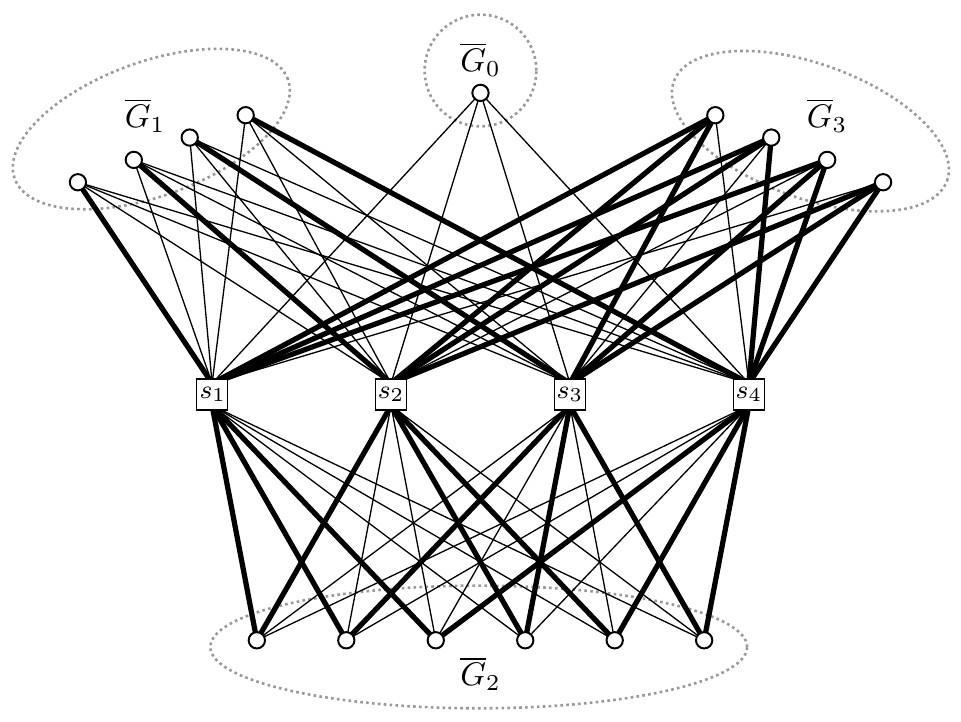
\includegraphics[width=0.6\textwidth]{images/k-server-advice.png}
    \caption{Konstruktion Graph für Beweis Advice-Komplexität von k-Server}
    \label{k-server-advice}
\end{figure}

\paragraph{Advice und Randomisierung}
Idee: Orakel muss zwar deterministisch sein, kann aber die Advice-Bits als die ``besten''
Zufallsbits wälen.

Wenn ein c-kompetitiver randomisierter OA existiert der $b(n)$ Zufallsbits liest,
so existiert auch ein c-kompetitiver OA mit Advice der $b(n)$ Advice-Bits liest, und vice versa.

Wenn \emph{kein} OA mit Advice existiert der $b(n)$ Advice-Bits liest,
so existiert auch \emph{kein} randomisierter OA der $b(n)$ Zufallsbits liest.

\paragraph{Satz (6.1)}
Sei $\Pi$ ein Online-Minimierungsproblem für das $m(n)$ verschiedene Instanzen der Länge $n$ existieren.
\footnote{Wir müssen die Anzahl der möglichen Eingaben einschränken.}
Sei $Rand$ ein randomisierter OA mit erwartetem kompetitiven Faktor $c$.

Dann existiert ein OA mit Advice der $((1 + \varepsilon) c)$-kompetitiv ist und Advice-Komplexität
$$\log \log (m(n))$$
hat. \footnote{Stark vereinfacht im Vergleich zum Skript.}
D.h. die Anzahl benötigter Advice-Bits hängt nur von der Anzahl Instanzen ab.

Umgekehrt: falls ein OA mit Advice mindestens mehr Advice-Bits braucht,
dann kann kein randomisierter OA existieren.
